\documentclass{article}
\input{def}
\begin{document}
\maketitle{Datalog for Static Analysis}

\begin{abstract}
These are post-lecture notes for my February 7th presentation for \href{http://www.ccs.neu.edu/home/matthias/7480-s17/index.html}{HOPL 2017}.
The theme is the use of Datalog as a framework for building static analyses.
The lecture covered the history of Datalog, who its original application to static analysis, and its later success.

These notes are a bare-minimum transcription of my on-paper notes for the lecture. Better than nothing.
\end{abstract}

\subsection*{Datalog for Static Analysis}

Last year, there were two new papers about an old domain-specific language.

\begin{itemize}
\item
{\emph{From Datalog to \flix}~\cite{myl-pldi-2016} at \href{http://conf.researchr.org/home/pldi-2016}{PLDI 2016}}
\item
{\emph{\datafun{}: A Functional Datalog}~\cite{ak-icfp-2016} at \href{http://conf.researchr.org/home/icfp-2016}{ICFP 2016}}
\end{itemize}
Both have a similar motivation, essentially:

\begin{quote}
  Datalog has been successful because it lies at a confluence between \emph{logic programming} and \emph{static analysis}.
\end{quote}
And both papers suggest new extensions for Datalog.
The goal today is to understand why and how Datalog has been successful.

To start, we'll trace the papers' citations.
Both cite work regarding the \href{http://www.logicblox.com/}{LogicBlox} Datalog engine: \flix\ cites the \doop\ program analyzer (for Java programs)~\cite{bs-oopsla-2009} and \datafun\ cites a paper that summarizes the engine~\cite{acgkopvw-sigmod-2015}.
They also both cite Whaley and Lam's \bddbddb{}.
Finally they each cite one early work on Datalog.
\flix\ cites Ullman's text on \emph{Principles of database and knowledge-base systems} and \datafun\ cites the proceedings of a 1978 workshop on Logic and Databases, hosted by Gallaire, Minker, and Nicholas.
(See \figref{fig:citations} for a picture of this paragraph.
The solid lines represent citations in the 2016 papers.)

At this point, the earliest cited work that ues Datalog to implement a static analysis is the \bddbddb{} paper, from 2004.\footnote{Ullman's text demonstrates how Datalog can express and solve the reaching definitions problem, that is likely the first work to present the \emph{idea} of implementing a static analysis with Datalog.}
The \bddbddb\ paper in turn cites work by Reps~\cite{r-ald-1994} that uses the \coral\ deductive database~\cite{rsss-sigmod-1993} (a Datalog database) to implement demand-driven program slicing.
But the idea of Datalog for static analysis goes (at least!) one step further: to Uwe \assmann{}'s dissertation work.

That's where we'll start today.
The road map is (1) \assmann{}, (2) classic Datalog, (3) \bddbddb, and (4) \doop{}.
In terms of deltas and contributions, we'll (1) see a uniform framework for expressing three static analyses, (2) rephrase that framework as Datalog, (3) see how context-sensitive points-to analysis turned Datalog from a novelty to a necessity, and (4) the power of a mature Datalog implementation.


% Here's the road map:
% \begin{enumerate}
% \item \emph{On Edge Addition Rewrite Systems And their Relevance to Program Analysis}, \assmann{}, 1994.
% \item \emph{What You Always Wanted to Know About Datalog}, Ceri, Gottlob, and Tanca, 1989. (My favorite reference on pure Datalog.)
% \item \emph{Context Sensitive Program Analysis as Database Queries}, Lam, Whaley, Livshits, Martin, Avots, Carbin, Unkel, 2004. (A \bddbddb\ paper.)
% \item \emph{Strictly Declarative Specification of Sophisticated Points-To Analyses}, Bravenboer, Smaragdakis, 2009. (The \doop\ paper.)
% \end{enumerate}

\begin{figure}[t]
  \begin{center}
  \begin{tikzpicture}
    \node[draw,shape=ellipse] (00) {\localpdf{myl-pldi-2016}{\flix{}, PLDI 2016}};
    \node[right of=00,xshift=3cm] (01) {};
    \node[draw,shape=ellipse,right of=01,xshift=3cm] (02) {\localpdf{ak-icfp-2016}{\datafun{}, ICFP 2016}};

    \node[below of=00,yshift=-0.5cm] (10) {};
    \node[draw,shape=ellipse,right of=10,xshift=2cm] (11) {\localpdf{acgkopvw-sigmod-2015}{LogiQL, SIGMOD 2015}};
    \node[right of=11] (12) {};

    \node[below of=10,yshift=-0.5cm] (20) {};
    \node[draw,shape=ellipse,right of=20,xshift=2cm] (21) {\localpdf{bs-oopsla-2009}{\doop{}, OOPSLA 2009}};
    \node[right of=21] (22) {};

    \node[below of=20,yshift=-0.5cm] (30) {};
    \node[draw,shape=ellipse,right of=30,xshift=2cm] (31) {\localpdf{wl-pldi-2004}{\bddbddb{}, PLDI 2004}};
    \node[right of=31] (32) {};

    \node[below of=30,yshift=-1cm] (40) {};
    \node[draw,shape=ellipse,right of=40,xshift=2cm] (41) {\localpdf{r-ald-1005}{Reps, CC 1994}};
    \node[draw,shape=ellipse,right of=41,xshift=2cm,yshift=-1cm] (42) {\localpdf{a-tagt-1994}{\assmann{}, TAGT 1994}};

    \node[draw,shape=ellipse,below of=40,yshift=-1.7cm] (50) {\localpdf{}{Ullman, \gbookhref{YmpqAAAAMAAJ}{1988}/\gbookhref{vUw1AQAAMAAJ}{1989}}};
    \node[right of=50,xshift=2cm] (51) {};
    \node[draw,shape=ellipse,right of=51,xshift=2cm,yshift=0.2cm] (52) {\localpdf{cgt-ieee-1989}{Ceri, Gottlob, Tanca, 1989}};

    \node[below of=50,yshift=-0.5cm] (60) {};
    \node[draw,shape=ellipse,right of=60,xshift=2cm] (61) {\emph{Logic and Databases}, Gallaire, Minker, Nicholas, 1978};
    \node[right of=61] (62) {};

    \draw[->] (00) edge[bend right=20] (21);
    \draw[->] (00) edge[bend right=30] (31);
    \draw[->] (00) -- (50);

    \draw[->] (02) -- (11);
    \draw[->] (02) edge[bend left=10] (31);
    \draw[->] (02) edge[bend left=60] (61);

    \draw[->,dashed] (11) -- (21);
    \draw[->,dashed] (21) -- (31);
    \draw[->,dashed] (31) -- (41);
    \draw[->,dashed] (41) -- (42);
  \end{tikzpicture}
  \end{center}
\hrule
\caption{Tracing citations}
\label{fig:citations}
\end{figure}


\subsection*{EARS}

\assmann{}'s framework for static analysis is EARS: Edge Addition Rewrite Systems.
His 1994 paper demonstrates how EARS can efficiently solve three problems in static analysis.


\subsubsection*{3 Static Analysis Problems}

\textbf{Basic Block Ordering} ({\bb}) is the problem of building a control-flow graph for a set of basic blocks.
\begin{itemize}
\item A \emph{basic block} is a straight-line sequence of machine instructions.
\item Every basic block has a unique label.
\item Machine instructions include definitions, jumps to other basic blocks, and conditional jumps to other basic blocks. (Jumps reference block labels.)
\item The last instruction in any basic block is a jump. Intermediate instructions are not jumps.
\item A control flow graph draws an edge from each basic block to its possible successors.
\end{itemize}

For example, the fragment of C code in \figref{fig:ears-c} might compile to three basic blocks.
%\begin{itemize}
The first would represent lines 2 and 3.
The second would represent line 4.
The third would represent line 5.
%\end{itemize}
A control flow graph would connect the first block to the other two, and the second block to the third.

\begin{figure}[t]
  \begin{lstlisting}[language=C,numbers=left,basicstyle=\tt,xleftmargin=.2\textwidth]
    int y,z;
    y = random();
    if (y > 0.5) {
       y = random();
    }
    z = 2 * y;
  \end{lstlisting}
\caption{Example C code.}
\label{fig:ears-c}
\end{figure}

\vspace{2ex}

\noindent\textbf{Reaching Definitions} ({\rd}) is the problem of associating variable references in a program with variable definitions.
In \figref{fig:ears-c}, the definition of {\tt y} on line 2 reaches the use on line 3.
The same definition also reaches line 6 because the first block (representing lines 2 and 3) is a direct predecessor of the third block (representing line 6).

To simplify this problem, \assmann\ assumes two relations between basic blocks and definition instructions.
\begin{itemize}
\item The \textsc{Def} relation associates basic blocks to definitions that exit the block.
      If a block defines the same variable twice, only the latter definition is in the \textsc{Def} relation.
\item The \textsc{Preserved} relation associates basic blocks to definitions; in particular, to definitions that the basic block does not overwrite.
\end{itemize}
These seem like big assumptions to me. Don't worry about it.

\vspace{2ex}

\noindent\textbf{Equivalence Classes / Value Numbering} ({\eq}) is the problem of finding \emph{syntactically equal} subexpressions within a basic block.
If the term {\tt x + y} occurs twice in a basic block, these two occurrences belong in an equivalence class.


\subsubsection*{Uniform Representation}

All three problems and their solutions can be expressed \emph{uniformly} as rewrite rules on graphs.
Figures~\ref{fig:ears-bb}, \ref{fig:ears-rd}, and \ref{fig:ears-eq} present \assmann{}'s rules.
Each rule has two parts: the left-hand side matches a sub-graph with labeled nodes and labeled edges (defined more formally in the next section).
The right-hand side adds one (or more) edges to the left-hand side graph.

\begin{figure}[t]
  \input{fig-bb.tex}
\caption{Graph rewrite system {\bb}}
\label{fig:ears-bb}
\end{figure}

\begin{figure}[th]
  \input{fig-rd.tex}
\caption{Graph rewrite system {\rd}}
\label{fig:ears-rd}
\end{figure}

\begin{figure}[t]
  \input{fig-eq.tex}
\caption{Graph rewrite system {\eq}}
\label{fig:ears-eq}
\end{figure}

For {\bb}, assume a \textsc{Last} relation associating basic blocks to their final (jump) instruction.
Then the rewrite rules to compute the ``successor'' relation between blocks are:
\begin{itemize}
\item ({\bb}-1) if the last instruction in block $B_1$ is a direct jump, the jump's target is a successor of $B_1$.
\item ({\bb}-2, {\bb}-3) if the last instruction in block $B_1$ is a conditional jump, the ``then'' and ``else'' targets are successors of $B_1$.
\end{itemize}
(\assmann\ simulataneously defines a ``predescessor'' relation between blocks.)

For {\rd}, assume the \textsc{Def} and \textsc{Preserved} relations noted above.
\begin{itemize}
\item ({\rd}-1) if a block defines a variable, the definition reaches the end of the block.
\item ({\rd}-2) if a definition flows into block $B_1$ and is not re-defined, the definition flows out of $B_1$.
\item ({\rd}-3) if a definition flows out of a block, it flows in to that block's successors.
\end{itemize}

For {\eq}, the goal is to compute ``shallow'' and ``deep'' equality relations (\textsc{Simple=} and \textsc{Tree=}, respectively).
These rules in \figref{fig:ears-eq} work for numbers and addition; any expression node $E$ is either a number or the sum of two expression nodes.
\begin{itemize}
\item ({\eq}-1) two number nodes with equal values are both \textsc{Simple=} and \textsc{Tree=}.
\item ({\eq}-2) any two sum nodes are \textsc{Simple=}.
\item ({\eq}-3) if two nodes are \textsc{Simple=} and have \textsc{Tree=} children, they are \textsc{Tree=}.
\end{itemize}

To find the solution of these problems on a program {\tt P}, first convert {\tt P} to an appropriate graphs and then apply the rewrite rules to a fixed point.


\subsubsection*{Termination and Strong Confluence}

The above graph rewrite systems are useful because they can \emph{express} a variety of static analysis problems and furthermore yield a terminating, strongly confluent algorithm for computing the solution.
Strong confluence means that applying the rewrite rules in \emph{any} order gives the same solution.

\assmann\ defines an \emph{edge-addition rewrite system} (EARS) $\mathcal{E}$ as a pair $(S, Z)$ where:
\begin{itemize}
\item $Z$ is a graph with labeled nodes, labeled edges, and a dictionary of attributes for each node.
  A given pair of nodes can have multiple edges between them, but each such edge must have a \emph{unique} label.
  Here is \assmann{}'s definition: $Z = \langle N, E, \Sigma_N, \Sigma_E, l_N, m_N, A_N\rangle$ where
  \begin{itemize}
  \item $N$ is a set of nodes
  \item $E$ is a set of triples $(N, N, \Sigma_E)$ (directed, labeled edges).
  \item $\Sigma_N$ is a set of node labels (e.g. a set of strings).
  \item $\Sigma_E$ is a set of edge labels.
  \item $l_N : N \mapsto \Sigma_N$ associates nodes to labels.
  \item $m_N : E \mapsto \Sigma_E$ associates edges to labels.\footnote{Seems redundant to me.}\footnote{I should point out: around this time in the presentation, Mitch said ``you all should look at a definition like this and, as scientists, pinpoint \emph{why it is wrong}.'' I think his point was, if the formalism isn't as simple and clear as possible, you need to fix the formalism.}\footnote{Around the same time, Olin said ``these compiler guys usually have a bunch of hacks and pseudo-math, and a very cool idea underneath''}
  \item $A_N$ is a set of functions that map nodes to a particular attribute.
    \assmann\ writes $A_N = \{ f \mid f : N \mapsto A_i, i \in \naturals \}$
  \end{itemize}
\item $S$ is a set of pairs of such graphs, such that $(G_L, G_R) \in S$ implies
 that $G_L$ and $G_R$ have the \emph{same nodes} and the edges of $G_L$ are a subset of the edges of $G_R$.
\end{itemize}
Intuition: $Z$ represents a program and $S$ is the graph rewrite rules.

Next, \emph{rule application} for an EARS is the non-deterministic process of selecting a rewrite rule in $S$ and applying it to $Z$.
Let $(S, Z) \rightarrow_R (S, Z')$ mean that applying rule $R \in S$ to graph $Z$ yield graph $Z'$.
\assmann\ states three conditions for $R \in S$ to apply to the EARS $(S, Z)$.
Let $R = (G_L, G_R)$:
\begin{enumerate}
\item There exists a graph morphism $g_L : G_L \rightarrow Z$.
\item The morphism $g_L$ preserves node attributes.\footnote{\assmann\ formalizes this. I won't.}
\item There is no morphism $g_R : G_R \rightarrow Z$ such that $g_L(G_L) \subseteq g_R(G_R)$.
\end{enumerate}
Condition 3 ensures that rule application adds an edge.
In other words, $(S,Z) \rightarrow_R (S,Z')$ implies that $Z$ is a strict subgraph of $Z'$.

\begin{theorem}
  the transitive closure of rule application is terminating and strongly confluent
\end{theorem}
\begin{proof}
Termination is obvious: rule application always adds an edge, and every graph contains at most one edge for every label and pair of nodes.

Confluence is also easy to prove, but relies on the reflexive-transitive closure of rule application, written $(S,Z) \rightarrow^* (S,Z')$.
Suppose there are two ways an EARS can step:
\begin{center}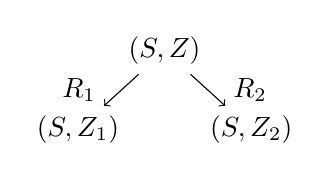
\begin{tikzpicture}
  \node (0) {$(S, Z)$};
  \node [below of=0] (1) {};
  \node [left of=1,xshift=-1mm] (2) {$(S, Z_1)$};
  \node [right of=1,xshift=1mm] (3) {$(S, Z_2)$};

  \draw[->] (0) -- node[left,xshift=-2mm] {$R_1$} (2);
  \draw[->] (0) -- node[right,xshift=2mm] {$R_2$} (3);
\end{tikzpicture}\end{center}

Then there exists an EARS $(S, Z_3)$ such that:

\begin{center}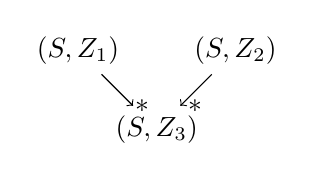
\begin{tikzpicture}
  \node (1) {};
  \node [left of=1] (2) {$(S, Z_1)$};
  \node [right of=1] (3) {$(S, Z_2)$};
  \node [below of=1] (4) {$(S, Z_3)$};

  \draw[->] (2) -- node[below right,xshift=1mm] {$*$} (4);
  \draw[->] (3) -- node[below left,xshift=2mm] {$*$} (4);
\end{tikzpicture}\end{center}

The proof is by cases on the edges added by $R_1$ and $R_2$.
Let these edges be the sets $E_1$ and $E_2$.
\begin{itemize}
\item If $E_1 = E_2$ then $Z_1 = Z_2 = Z_3$. Do nothing.
\item If $E_1 \subset E_2$ then $Z_2 = Z_3$. Apply $(S, Z_1) \rightarrow_{R_2} (S, Z_3)$.
\item If $E_2 \subset E_1$ then $Z_1 = Z_3$. Apply $(S, Z_2) \rightarrow_{R_1} (S, Z_3)$.
\item Otherwise, apply $(S, Z_1) \rightarrow_{R_2} (S, Z_3) {}_{R_1}\leftarrow (S, Z_2)$.
\end{itemize}
\end{proof}


\subsubsection*{Efficent Solutions}

These problems ({\bb}, {\rd}, {\eq}) are old problems in static analysis.
When \assmann{} began developing his framework, all three problems had well-known and efficient solutions.
But the solutions for each problem were ad-hoc; it was not clear how those solutions could systematically lead to efficient solutions for other problems.

The main contribution of the EARS framework is that it provides a \emph{systematic} method of deriving \emph{efficient solutions} to problems.
\assmann\ shows that these solutions are as efficent as the previously-known, ad-hoc solutions.
See the paper for details: the idea is to start with a straightforward, iterative solution and optimize the for-loops based on the number of nodes in a rewrite rule with no incoming edges.


\subsubsection*{To Datalog}

In a short subsection, \assmann\ notes that his graph rewrite rules can be mapped to Datalog.
EARS are ``just Datalog'', and Datalog is ``just EARS''.
The next section introduces Datalog and explains the mapping.


\subsubsection*{EARS External Links}
\begin{itemize}
\item Sourceforge page for Optimix: \url{http://optimix.sourceforge.net/}
  Optimix is part of \assmann{}'s dissertation, it is a language for specifying EARS-based transformations for C and Java code.
\item DBLP page for the TAGT conference (where the EARS paper appeared): \url{http://dblp.uni-trier.de/db/conf/gg/index.html}
\end{itemize}


\subsection*{Datalog}

One quick definition of Datalog is ``\prolog\ without function symbols or negation''.
Another is ``a deductive database''; that is, a database extended with first-order Horn clauses.

\begin{figure}[t]
  \begin{center}$\begin{array}{l l l}
    S & \coloneq & R \ldots
    \\
    R & \coloneq & F \mid Q \mid L \colondash L \ldots
    \\
    F,Q,L & \coloneq & p(a\ldots)
    \\
    p & \coloneq & \langle {\tt symbol} \rangle
    \\
    a & \coloneq & \langle {\tt symbol} \rangle \mid X
  \end{array}$\end{center}
  \caption{Datalog syntax}
  \label{fig:datalog-syntax}
\end{figure}

\figref{fig:datalog-syntax} presents a syntax for Datalog.
A program $S$ is a sequence of facts $F$, rules, and queries $Q$.
A rule $L_0 \colondash L_1 \ldots L_n$ is an axiom for deducing new information ($L_0$) from existing facts ($L_i$, for $i \in [1,n]$).
Facts, rules, and queries consist of predicate symbols $p$ and atoms $a$.
Atoms are either symbols (typeset in $\dlp{lowercase, serif}$ font) or variables (captalized, in math mode, e.g. $\dlv{X}$).

There are two syntactic restrictions:
\begin{enumerate}
\item A fact may not contain variables.
\item Any free variables in the head of a rule must be appear in the rule's body.
  Let $\fvs{L}$ denote the set of variables that appear in $L$.
  Then the restriction on $L_0 \colondash L_1 \ldots L_n$ is that $\fvs{L_0} \subseteq \bigcup_{i \in [1,n]} \fvs{L_i}$.
\end{enumerate}

\begin{figure}
  \begin{center}$\begin{array}{l l l}
  %\dlp{basic\_block}(\dlp{b_1})
  %& \dlp{instruction}(\dlp{i_3})
  %& \dlp{last}(\dlp{b_1}, \dlp{i_3})
  %\\
  %\dlp{basic\_block}(\dlp{b_2})
  %& \dlp{kind}(\dlp{i_3}, \dlp{jump})
  %&
  %\\
  %\dlp{lbl}(\dlp{b_2}, \dlp{l})
  %& \dlp{lbl}(\dlp{i_3}, \dlp{l})
  %&
  %\\
  %& &
  %\\
  \dlp{b\_succ}(\dlv{B_0}, \dlv{B_1}) \colondash
  & \dlp{basic\_block}(\dlv{B_0})
  &
  \\
  & \dlp{basic\_block}(\dlv{B_1})
  &
  \\
  & \dlp{last}(\dlv{B_0}, \dlv{I})
  &
  \\
  & \dlp{kind}(\dlv{I}, \dlp{jump})
  &
  \\
  & \dlp{lbl}(\dlv{I}, \dlv{L})
  &
  \\
  & \dlp{lbl}(\dlv{B_1}, \dlv{L})
  &
  \end{array}$\end{center}
  \caption{Datalog encoding of {\bb}-1}
  \label{fig:datalog-bb}
\end{figure}

\figref{fig:datalog-bb} encodes the rule {\bb}-1 in Datalog.
This encoding assumes there are predicates $\dlp{basic\_block}$, $\dlp{last}$, $\dlp{kind}$, and $\dlp{lbl}$ corresponding to the edges and labels in the {\bb}-1 graph.
Using these predicates, the rule describes how to deduce that a block $B_0$ has a successor block $B_1$.

The syntax and example should give an intuition for the semantics of a Datalog program.
For one last bit of intuition, here is the translation ($\sim$) of a Datalog rule to first-order logic (specifically, a translation from rules to Horn clauses):


\[
  L_0 \colondash L_1 \ldots L_n
  \sim
  \forall \vec{X}\,.\,(L_1 \wedge \ldots \wedge L_n) \Rightarrow L_0
\]

\[
  \mbox{where } \vec{X} = \bigcup_{j \in [0,n]} \fvs{L_j}
\]

More precisely, the semantics of a Datalog program is the least fixed point of the \emph{elementary production principle} (EPP).
The EPP describes how a Datalog program $S$ can step to a program $S'$ using a rule in $S$ to derive a new fact:

\begin{center}$\begin{array}{l l l}
  S \rightarrow_R (S \cup (L_0~\theta))
  & \iff & \exists R \in S
  \\ & & \wedge~R = L_0 \colondash L_1 \ldots L_n
  \\ & & \wedge~\exists F_1 \ldots F_n \in S
  \\ & & \wedge~\vec{X} = \bigcup_{j\in [0,n]} \fvs{L_j}
  \\ & & \wedge~\exists \theta : \vec{X} \mapsto F \mbox{ such that } \theta(X) \in S
  \\ & & \wedge~\forall i \in [1,n]\,.\, L_i~\theta = F_i
\end{array}$\end{center}
\noindent where $L~\theta$ is the fact produced by replacing free variables in $L$ by their value in $\theta$.

The least fixed point of applying the EPP is the set of facts that a Datalog program represents.


\subsubsection*{Databases}

The previous section explains how a Datalog program $S$ represents a database of facts.
This database is known as the \emph{intensional database} (or IDB) represented by $S$~\cite{cgt-ieee-1989}.

It's often useful to connect a Datalog program to an existing database of facts.
Such databases are called \emph{extensional databases}.

Once we incorporate an extensional database, we can view a Datalog program $P$ as a mapping from an EDB to an IDB:

\[ P : \mbox{EDB} \rightarrow \mbox{IDB} \]

Typically, $P$ is a \emph{time-invariant} mapping from a \emph{time-invariant} set of facts (the EDB) to some answer (the IDB).

(The EDB / IDB distinction is a pragmatic one. You could pretend that the EDB is a sequence of facts at the top of the Datalog program and the IDB is always fully computed and committed to an extensional database.)


\subsubsection*{History Lesson}

My reference for ``pure Datalog'' is the 1989 article by Ceri, Gottlob, and Tanca~\cite{cgt-ieee-1989}.
At that time, Datalog was well-known and well understood in the \emph{logic and databases} community.
Here's a very quick timeline of the world until 1989.

\begin{itemize}
\item (19XX) databases are as old as computers.
  The early implementations\footnote{Such as IBM's \href{https://en.wikipedia.org/wiki/Hierarchical_database_model}{hierarchical model}.} were \emph{link-based}.
  Unlike computers, there was no early mathematical model of databases.
\item (1970) Codd proposed the \emph{relational model} of databases, founded on \emph{relational algebra}~\cite{c-cacm-1970}.
  This was a hit.
  For example, \textsf{SQL} databases are relational databases.
  Codd received a Turing award in \href{http://amturing.acm.org/award_winners/codd_1000892.cfm}{1981}.
\item (196X-197X) meanwhile, researchers began exploring the idea that mathematical logic could be useful for understanding databases.
\item (1973) Colmeraur and his students develop the first \prolog\ interpreter.
\item (1974) Kowalski suggests logic as a programming language.
\item (1976) Van Emden and Kowalski give a semantics of predicate logic as a programming langauge~\cite{vk-jacm-1976}.
  Datalog \emph{is} predicate logic; their model-theoretic, proof-theoretic, and fixpoint semantics were the foundation.
\item (1978) Gallaire, Minker, and Nicholas organized a workshop titled \emph{Logic and Databases}.
  At this workshop:
  \begin{itemize}
  \item Someone introduced Datalog.
  \item Reiter stated the \emph{closed-world axiom} implicit in relational models.
  \item Clark stated the \emph{completion axiom}, also implicit in relational databases.
  \end{itemize}
\item (198X) researchers explored extensions to Datalog and techniques for efficiently answering queries (without computing the entire IDB!).
  Extensions include:
  \begin{itemize}
  \item negation
  \item arithmetic, primitive functions such as {\tt <}
  \item complex objects, missing information {\tt null}
  \end{itemize}

  Evaluation techinques include:
  \begin{itemize}
  \item semi-na\"ive evaluation
  \item the magic sets transformation
  \item the query-subquery method
  \end{itemize}
\end{itemize}

Suffice to say, Datalog was considered a successful experiment by 1989.
No commercial implementations of Datalog existed, but the theory was all laid out.

In fact, the magic sets transformation is the premise of the 1994 paper by Reps~\cite{r-ald-1994}.
The transformation minimizes the number of facts computed to answer a query based on symbols that appear in the query.
Reps uses this transformation to implement \emph{demand-driven} program slicing.

\emph{One more thing that doesn't fit anywhere else:} Datalog corresponds to \emph{positive relational algebra} with recursion.
Full relational algebra has a set-difference operator.

\emph{One more thing:} I posit that there is a paper that proves you can encode any polynomial time algorithm in Datalog~\cite{degv-csur-2001}.
(\flix{} cites this paper as such, but I did not understand the paper's theorems.)

\subsubsection*{Further Reading}
\begin{itemize}
\item The survey by Gallaire, Minker, and Nicholas~\cite{gmn-csur-1984}.
\item The 20-year retrospective by Minker~\cite{m-lfca-1999}.
\end{itemize}


\subsection*{Context-sensitive Points-To Analysis (for Java)}

\assmann\ and Reps demonstrated that Datalog could successfully be used to implement static analyses.
Very good.
But for the next decade, there doesn't seem to be much work using Datalog for static analysis.\footnote{Mitch says: that's not entirely true, there are definitely some papers where---if you squint---you realize they're using Datalog.}

(As I understand, \assmann\ didn't use Datalog because (1) his goal was to add EARS to an existing compiler, which used adjacency lists as an IR and (2) he did not have access to a Datalog implementation.
Reps used the \coral\ deductive database, but reported order-of-magnitude slowdowns for using \coral\ rather than C.)

It took the combination of an old problem and a new programming paradigm to revive interest.
The paradigm was object-oriented programming.
The problem was context-sensitive points-to analysis.

Points-to analysis is essentially the reaching definitions ({\rd}) problem.
The goal, in the OOP sense, is to describe the heap objects that a variable can denote.
A context-sensitive points-to analysis further indexes this information.
Exactly how to index is a design choice; for example, one way to index is to track the previous three (generalization: $k$) method names on the call stack.

\emph{Proposition:} many static analyses require points-to information.

In the early 2000's, if you wanted points-to information for your Java program, you had essentially two alternatives:
\begin{itemize}
\item Apply a know context-sensitive algorithm, limit yourself to programs of about 3,000 lines.
\item Apply a unification-based~\cite{s-popl-1995} or context-insensitive algorithm.
\end{itemize}


\subsubsection*{Scaling Points-to Analysis}

John Whaley and (advisor) Monica Lam at Stanford came up with a radical solution~\cite{wl-pldi-2004}.
They decided to apply a context-\emph{insensitive} algorithm to an \emph{exploded} control-flow graph.
That is, they added paths to a given control-flow graph to make context information explicit in the paths.
Consequently, the insensitive algorithm would give context-sensitive results.

The obvious problem with this approach is that the number of contexts in a large, object-oriented program is usually large.\footnote{This is exactly why previous algorithms did not work at scale.}
Whaley and Lam report that $10^{14}$ contexts is ``typical'', and one of the DaCapo benchmarks had $10^{23}$ contexts.\footnote{A context is a call path to a method, e.g. they are reporting that if you count all the paths to all the methods, it's typical that the total count is $10^{14}$. A second, common kind of context-sensitivity is \emph{object sensitivity}~\cite{sbl-popl-2011}. Thank you to \href{http://rgrig.appspot.com/}{Radu Grigore} for helping me understand the contexts.}
Yet they made the algorithm work at scale by:
\begin{itemize}
\item representing program paths as relations
\item representing relations as boolean functions
\item using binary decision diagrams (BDDs)~\cite{a-ieee-1978} to efficiently represent the functions.
\end{itemize}
\noindent BDDs worked because these contexts had a lot of redundant information.

\subsubsection*{Datalog for Points-to Analysis}

The PLDI 2004 paper~\cite{wl-pldi-2004} reports on the implementation of \bddbddb{}: a binary-decision-diagram based deductive database.
The database front-end is Datalog.
Whaley and Lam encoded a points-to of C and Java programs as Datalog rules.
(Later, with Livshits, Martin, Avots, Carbin, and Unkel, they encoded a variety of taint analyses in Datalog~\cite{lwlmacu-pods-2005}.\footnote{And \emph{furthermore} developed a compiler from source-code patterns to Datalog rules.})

The database back-end is binary decision diagrams.
That's right, Whaley and Lam built an efficient deductive database from the ground up just to implement points-to analysis.

Conclusion: they succeeded at a problem that nobody before they could solve.
Their points-to analysis finished in minutes on programs selected from the DaCapo benchmarks~\cite{bghkmbdffghhjlmpsvvw-oopsla-2006}.\footnote{Remember that program with $10^{23}$ contexts? Well \bddbddb\ could not actually encode all those, it stopped at $2^{64} - 1$ contexts and merged all others into the last context.}


\subsection*{A Commercial Datalog Engine}

Finally, I want to mention the \doop\ system for points-to analysis of Java programs~\cite{bs-oopsla-2009}.
\doop\ builds on \bddbddb\ and the later \paddle\ system~\cite{lh-tosem-2008} in that \doop\ is:
\begin{itemize}
\item encodes call-graph construction in Datalog (as well as the points-to analysis);
\item extends the logic from the \paddle\ system~\cite{lh-tosem-2008} to encode more details of the Java language;
\item handles reflection ``better'' (details were not apparent to me);
\item handles exceptions ``better'' by building the relevant parts of the call graph\footnote{I think this is possible because the \doop\ builds a call graph on-demand instead of pre-computing, similar to how Reps used Datalog for demand-driven program slicing. But this is just a guess, beyond the phrase ``on-the-fly'' the details were not apparent to me from reading the paper.}
\end{itemize}

\doop\ is historically significant because it uses a commercial Datalog engine developed by \href{http://www.logicblox.com/}{LogicBlox}.

I am not aware of any work before \doop\ to mark the existence of a commercial (i.e. implementing all the optimizations from the 1980's) Datalog engine.
That means its approximately 33 years from the initial conference on logic and databases to a practical realization.

Oh, and by modifying their Datalog rules to trigger certain behavior in the Datalog engine, Bravenboer and Smaragdakis achieve numbers that suggest \doop\ is the fastest and most scalable implementation of points-to analysis for Java programs.
Regarding scalability, they are able to index each pointer with 2 abstract objects or associate 2 contexts to each heap location.
The \paddle\ system implemented these settings, but did not produce results in reasonable time.


\subsection*{Conclusions}

Datalog is:
\begin{itemize}
\item predicate logic as a programming language
\item a convenient interface to a database
\end{itemize}

The high-level benefits of storing program facts in a database and encoding a static analysis in Datalog are:
\begin{itemize}
\item the encoding works for a variety of problems, and yields a uniform solution
\item the Datalog encoding separates the \emph{specification} of the analysis from \emph{how to compute} the analysis
\item techniques for efficient evaluation of Datalog are techniques for efficient evaluation of your analysis
\end{itemize}

Meta-lessons: watch out for
\begin{itemize}
\item confluence points among research areas
\item sub-Turing languages that solve a real problem
\end{itemize}


\subsection*{FAQ}

(Not really an FAQ. These are the questions I had answers to prior to the talk, and my answers to questions that came up at the end.)


\qa{
  Does the \bddbddb\ paper report the overhead of building the deductive database?
}{
  Not that I know of.
  I do know that the \doop\ paper criticizes the overhead of BDDs~\cite{bs-oopsla-2009}, so lets say it's ``significant'', but not outrageous.

  The \textsc{Averroes} paper later criticized the overhead of representing a program analysis in \doop{}~\cite{al-ecoop-2013}.
  So it goes.
}

\qa{
  Given the overhead, do you still think Datalog is a good idea.
}{
  Yeah I think this is ``the future''.
  Data is cheap, and we should look to re-use quality research (e.g. evaluation techniques for Datalog) without reinventing them each time (building a \bddbddb{}).
}

\qa{
  Is there an easy way to try or use Datalog?
}{
  Yes.
  There's implementations everywhere.
  You can play with \href{http://docs.racket-lang.org/datalog/datalog.html}{{\tt \#lang datalog}} in Racket.
  For real work,
   there's the \href{http://www.datomic.com/}{Datomic} library for Clojure,
   \href{https://graphik-team.github.io/graal/}{Graal} project for Java,
   and \href{https://github.com/nwf/dyna}{Dyna} for Haskell.
  Also see the recent work on \href{https://github.com/flix}{\flix} and \href{https://github.com/rntz/datafun}{\datafun}.
}

\qa{
  Why did you pick this topic?
}{
  Last Spring I was building on the Type Systems as Macros~\cite{ckg-popl-2017} approach to type systems to put static analysis in the Racket macro expander.
  Researching Datalog is a step in a broader goal of looking at other frameworks for static analysis to determine what will work best in the macro expander.
}

\qa{
  Can you quickly explain this magic sets thing?
}{
  Sure, it's a source-code rewriting technique.
  Start with a query, for example $\dlp{p}(\dlp{a}, \dlv{X})$.
  Then rewrite the $\dlp{p}(\dlv{A},\dlv{B})$ rule to include the condition $\dlp{relevant}(\dlv{A})$.
  If $\dlv{A}$ is not relevant, you don't want to compute facts about it.
  This ``$\dlp{relevant}$'' predicate is a new rule that's introduced by the rewriting, along with the fact $\dlp{relevant}(\dlv{a})$ and some way of identifying other relevant atoms.
}

\qa{
  Any opinions on \flix{} and \datafun{}?
}{
  \flix{} sounds exicting.
  It's not straightforward to express lattice-based program analysis in Datalog.
  It is straightforward to do so in \flix{}.

  What worries me though, is that they're building a Datalog engine from scratch.
  Hope they stick with it, and implement the optimizations.

  \datafun{} is interesting, but I need to see more (or read the paper more carefully).
  For example, they cite other researchers extensions to Datalog as evidence that we could use a typed functional language for implementing Datalog extensions.
  But they don't show whether the language can express those existing extensions.
}

\qa{
  Final remarks?
}{
  There's an interesting ``wishlist'' at the end of the Ceri, Gottlob, Tanca article~\cite{cgt-ieee-1989}:
}
  \begin{itemize}
  \item To date, there are no useful applications of recursive or non-linear Datalog rules (points-to analysis certainly changed that)
  \item Datalog would be more useful if it was more of a programming language, e.g. with modules and structures, and the ability to implement a user interface. (Shouts out to \datafun{}.)
  \item Datalog is too declarative, sometimes you really do want to go low-level and control how things compute.
  \item Datalog focuses on interactions with a single database, but the modern trend is towards heterogenous systems.
  \end{itemize}
\noindent They thought about a lot of interesting things in 1989.

\footnotesize
\bibliographystyle{plain}
\bibliography{datalog-for-static-analysis}
\end{document}
